\section{问题四模型的建立与求解}
\label{sec:problem4}

\subsection{问题分析与建模思路}

问题四要求把前三问在交叉熵 Loss 尺度上的资源配置结论转换为可比较的下游能力，并进一步回答两个问题：开源大语言模型的历史能力提升有多少与训练规模扩张相关，有多少表现为控制已观测规模后的非规模残余；当训练算力增速放缓时，未来 $12$ 个月和 $24$ 个月的能力前沿将如何变化。已有研究表明，规模扩张与训练算法改进都能推动语言模型性能提升，但预训练 Loss 不能完全解释下游表现，相同 Loss 的模型仍可能具有不同的迁移能力\cite{ho2024algorithmicprogress,liu2023samepretraining}。因此，本文不把 Loss、训练算力与 Benchmark 视为可无误差互换的同一指标，而是建立带有支持域标记和不确定性传播的分层模型。

附件 C 的三类证据在样本规模和可比程度上差异明显。C1/C2 提供统一六任务口径的大样本能力面板，C4 提供较稀疏但可追溯的训练算力和开放权重证据，C6 则提供 Loss 与 Benchmark 的局部配对。若将三类记录直接拼接，既会重复计算同一排行榜记录，也会把桥接预测误当成历史观测。为此，本文依次完成能力量表重建、Loss--Benchmark 单调桥接、动力学能力前沿拟合、贡献分解和算力情景预测；问题三的 $45$ 个冻结方案只在桥接完成后映射为能力情景，不进入历史前沿训练集。

本文采用观察性动力学分解而非严格因果推断。后文所称“规模扩张相关贡献”指模型中训练算力变化对应的预测增量；“非规模残余技术贡献”是控制已观测规模后的时间状态增量，其中仍可能包含数据、架构、优化、后训练及未观测混杂，不能等同于纯算法进步。

\subsection{输入、数据与证据边界}

\subsubsection{数据去重、开放口径与模型分层}

主能力面板优先使用 C2，并以 C1 核验六项得分。原始 $4576$ 条记录经版本级去重后保留 $4546$ 条；主时间轴取提交日期，其有效范围为 2024 年 6 月 8 日至 2025 年 3 月 13 日。开放口径要求 C2 或高置信 C4 匹配明确给出开放权重证据；严格敏感性还要求许可证允许研究和复现，许可证缺失不自动视为 unrestricted。模型类型分为 pretrained、posttrained、merge 和 excluded，确认性贡献分解只使用 pretrained 与 continuously pretrained，以避免将微调收益或基座算力重复归入预训练规模。

C1/C2 与 C4 的实体匹配同时核对规范化名称、组织、模型族、版本和参数量。由此接受 $66$ 条 C4 匹配，最终得到 $41$ 条确认性前沿样本，覆盖 $7$ 个有效月份和 $13$ 个模型家族。posttrained 层仅有 $6$ 条合格算力记录，未达到独立分解所需的支持度，故只作样本覆盖说明而不强行拟合后训练贡献。各附件的使用方式见表~\ref{tab:p4_data_roles}。

\begin{table}[htbp]
\centering
\caption{问题四主要数据源、有效规模与建模角色}
\label{tab:p4_data_roles}
\small
\setlength{\tabcolsep}{4pt}
\begin{tabular}{p{0.12\textwidth}p{0.18\textwidth}p{0.25\textwidth}p{0.35\textwidth}}
\toprule
数据源 & 有效规模 & 主要作用 & 去重或降级规则 \\
\midrule
C1/C2 & 原始 $4576$ 条，去重后 $4546$ 条 & 六任务官方能力、提交日期、模型类型与许可证 & C2 为主表，C1 只核验分数；同版本重复提交保留最后一次有效记录 \\
C3 & $26$ 条历史论文/报告记录 & 长期方向敏感性 & $4573$ 条同源排行榜记录不与 C1/C2 重复计权 \\
C4 & $3523$ 条原始记录，接受匹配 $66$ 条 & 训练算力、数据量、开放权重和证据层 & Benchmark 反推算力不进入主模型；确认性前沿保留 $41$ 条 \\
C5/C6 & $43/75$ 条 & Loss--Benchmark 桥接 & C5 是 C6 子集，只用 C6 拟合一次 \\
C8 & $1863$ 个模型目录 & BBH/MATH 逐任务重算 & BBH 通过正式复现；MATH 未过门槛，仅作审计敏感性 \\
问题三接口 & $45$ 个冻结情景 & 将最优 Loss 映射为多维能力 & 保持情景与证据标签不变，不进入历史前沿训练 \\
\bottomrule
\end{tabular}
\end{table}

图~\ref{fig:p4_data_audit} 汇总了从原始记录到确认性面板的筛选链，并将 BBH、MATH 的逐任务复现结果与数据保留率并列展示。该审计图说明后续前沿估计使用的是通过实体匹配、证据分层和复现门槛共同筛选后的样本，而非直接使用全部排行榜记录。

\begin{figure}[H]
  \centering
  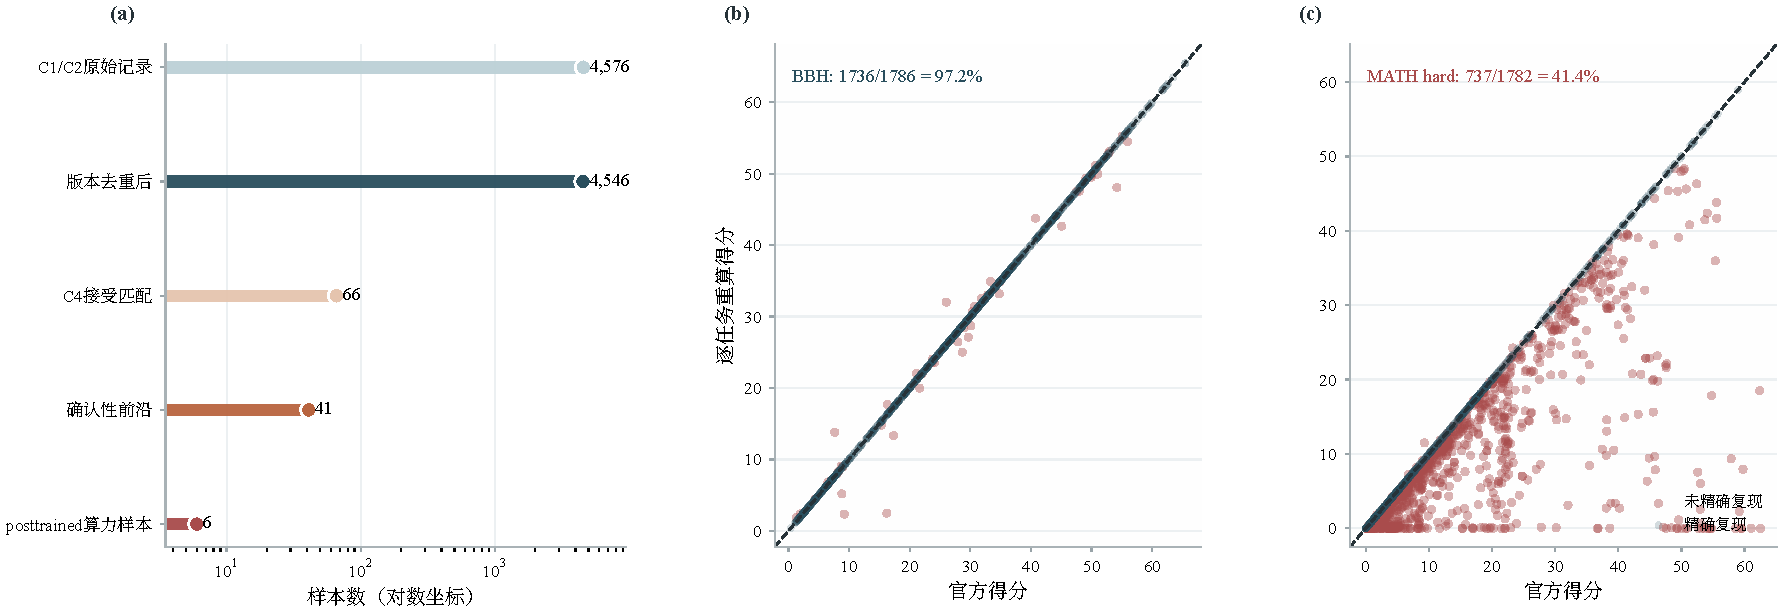
\includegraphics[width=0.98\textwidth]{images/no4/P4_F01_数据筛选与逐任务复现审计.pdf}
  \caption{问题四的数据筛选与逐任务复现审计}
  \label{fig:p4_data_audit}
\end{figure}

\subsubsection{综合能力与逐任务复现}

以六项官方归一化得分的算术均值定义模型 $i$ 的综合能力：
\begin{equation}
S_i^{\mathrm{avg}}=\frac{1}{6}\sum_{k=1}^{6}S_{ik},
\label{eq:p4_average_score}
\end{equation}
其中六项任务为 IFEval、BBH、MATH、GPQA、MUSR 和 MMLU-PRO。复算结果与官方 Average 的最大绝对误差为 $1.421\times10^{-14}$，说明量表闭合。为避免验证期信息泄漏，六维秩正态平衡分只作为敏感性指标，其经验分布函数始终在当期训练窗内估计。

根据 Open LLM Leaderboard 的官方归一化规则\cite{huggingface2024normalization}，BBH 的每个子任务须先扣除随机猜测下界，再对子任务等权平均。设模型 $i$ 在子任务 $j$ 上的原始分数为 $s_{ij}$，随机下界为 $l_j$，则
\begin{equation}
z_{ij}=\max\left\{0,\frac{s_{ij}-l_j}{1-l_j}\right\},\qquad
\widehat S_i^{\mathrm{BBH}}=\frac{100}{|J_i|}\sum_{j\in J_i}z_{ij}.
\label{eq:p4_bbh}
\end{equation}
在 $1786$ 个唯一可比模型中，重算 BBH 与官方分数精确一致的模型为 $1736$ 个，占 $97.2\%$，超过预注册的 $95\%$ 门槛。MATH hard 仅精确复现 $737/1782$，未达到门槛，故不作为正式逐任务复现证据。这一降级不会改变式~\eqref{eq:p4_average_score} 的官方综合能力主表。

\subsection{模型建立}

\subsubsection{Loss--Benchmark 单调桥接}

\subsubsection{有界变换与候选映射}

Loss 与下游能力虽总体负相关，但不同数据分布、模型族和离散任务转换会削弱这种关系；相同预训练 Loss 也可能对应不同的下游表现\cite{gadre2025scalereliably,liu2023samepretraining,schaeffer2025predicting,mayilvahanan2025line}。为保证能力预测自然落在 $0$--$100$，定义严格互逆的有界变换
\begin{equation}
g_{\epsilon}(S)=\operatorname{logit}\left(\frac{S+\epsilon}{100+2\epsilon}\right),\qquad
g_{\epsilon}^{-1}(y)=(100+2\epsilon)\sigma(y)-\epsilon,
\quad \epsilon=0.5,
\label{eq:p4_link}
\end{equation}
其中 $\sigma(\cdot)$ 为 Logistic 函数。该变换在 $0,5,50,99,100$ 五个校验点上的最大往返误差为 $1.421\times10^{-14}$。

对综合能力与六项任务分别拟合
\begin{equation}
g_{\epsilon}(S_{im})=h_m(\log L_i)+e_{im},
\qquad \frac{\mathrm d h_m(x)}{\mathrm dx}\le0,
\label{eq:p4_bridge}
\end{equation}
其中 $L_i$ 为验证 Loss，$h_m$ 为常数、单调线性、低自由度单调样条或保序回归之一。高可比记录权重为 $1$，中可比记录主权重为 $0.25$；按来源族留一验证计算 MAE、RMSE、Spearman 相关、区间覆盖率和区间宽度，并在最优 MAE 的一个标准误差内选择最简单模型。

Average 最终选择单调线性桥接，其 $12$ 个来源族折外 MAE 为 $10.217$、RMSE 为 $12.387$，优于常数基线 MAE $11.383$。IFEval、MATH 和 GPQA 未稳定优于常数基线，标记为弱桥接目标，不能承担综合能力主结论。完整桥接支持域为 Loss $1.65$--$2.84$，其中严格高可比范围为 $2.0933$--$2.5978$；范围外预测必须带外推标签，不作无标识延伸。

图~\ref{fig:p4_bridge_validation} 展示 one-SE 选模及留来源族验证结果，图~\ref{fig:p4_bridge_models} 则横向比较七类能力目标的候选桥接误差。二者共同支持“综合能力采用单调线性桥接、弱目标降级使用”的选择。

\begin{figure}[H]
  \centering
  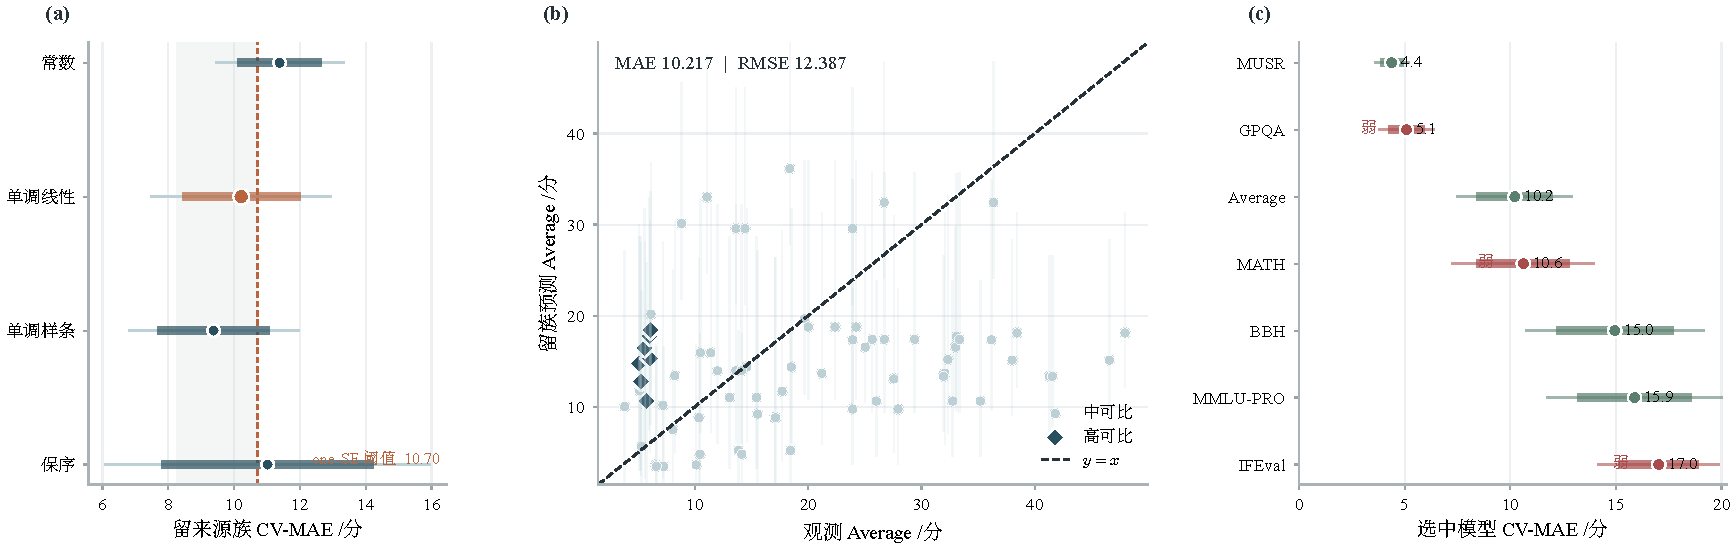
\includegraphics[width=0.99\textwidth]{images/no4/P4_F02_Loss_Benchmark桥接选择与留族验证.pdf}
  \caption{Loss--Benchmark 桥接的 one-SE 选模与留来源族验证}
  \label{fig:p4_bridge_validation}
\end{figure}

\begin{figure}[H]
  \centering
  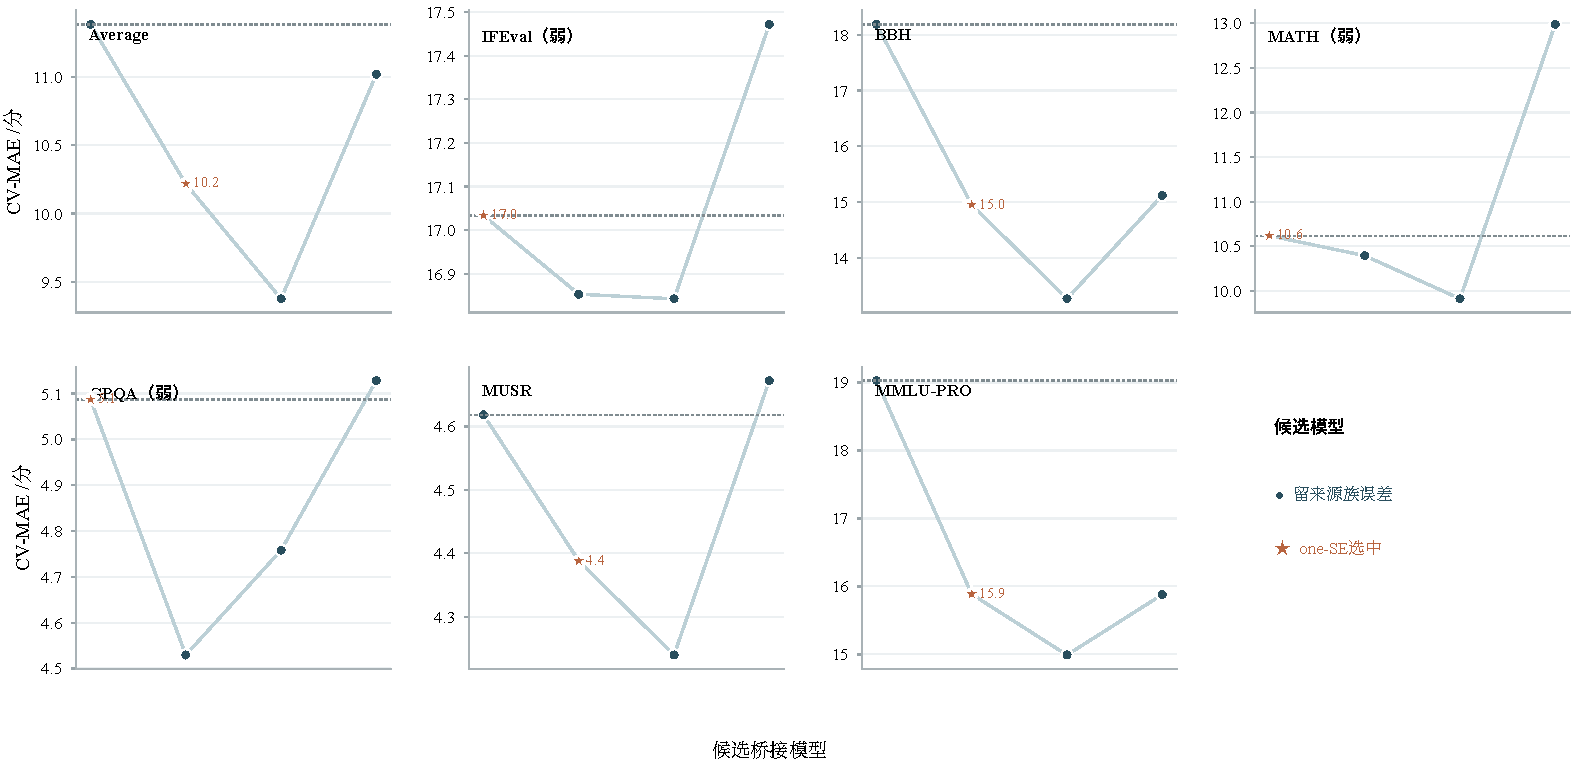
\includegraphics[width=0.97\textwidth]{images/no4/P4_A01_七类能力桥接模型比较.pdf}
  \caption{七类能力目标的候选桥接模型留来源族误差}
  \label{fig:p4_bridge_models}
\end{figure}

\subsubsection{问题三方案的能力映射}

问题三的每个 Loss bootstrap 样本与桥接来源族 bootstrap 配对传播，分别形成仅上游、仅桥接和联合三组区间。$45$ 个情景中，$15$ 个为高支持、$15$ 个为扩展支持、$15$ 个超出桥接范围。以正文主情景 $L_{\mathrm{ctx}}=4096$ 为例，三类质量成本下的综合能力映射见表~\ref{tab:p4_p3_mapping}。

图~\ref{fig:p4_p3_mapping} 先给出全部问题三方案从 Loss 到综合能力的连续映射，再由表~\ref{tab:p4_p3_mapping} 报告代表性预算点的数值和支持标签。图表并用可避免将范围外方案与高支持方案混为同等可信度。

\begin{figure}[H]
  \centering
  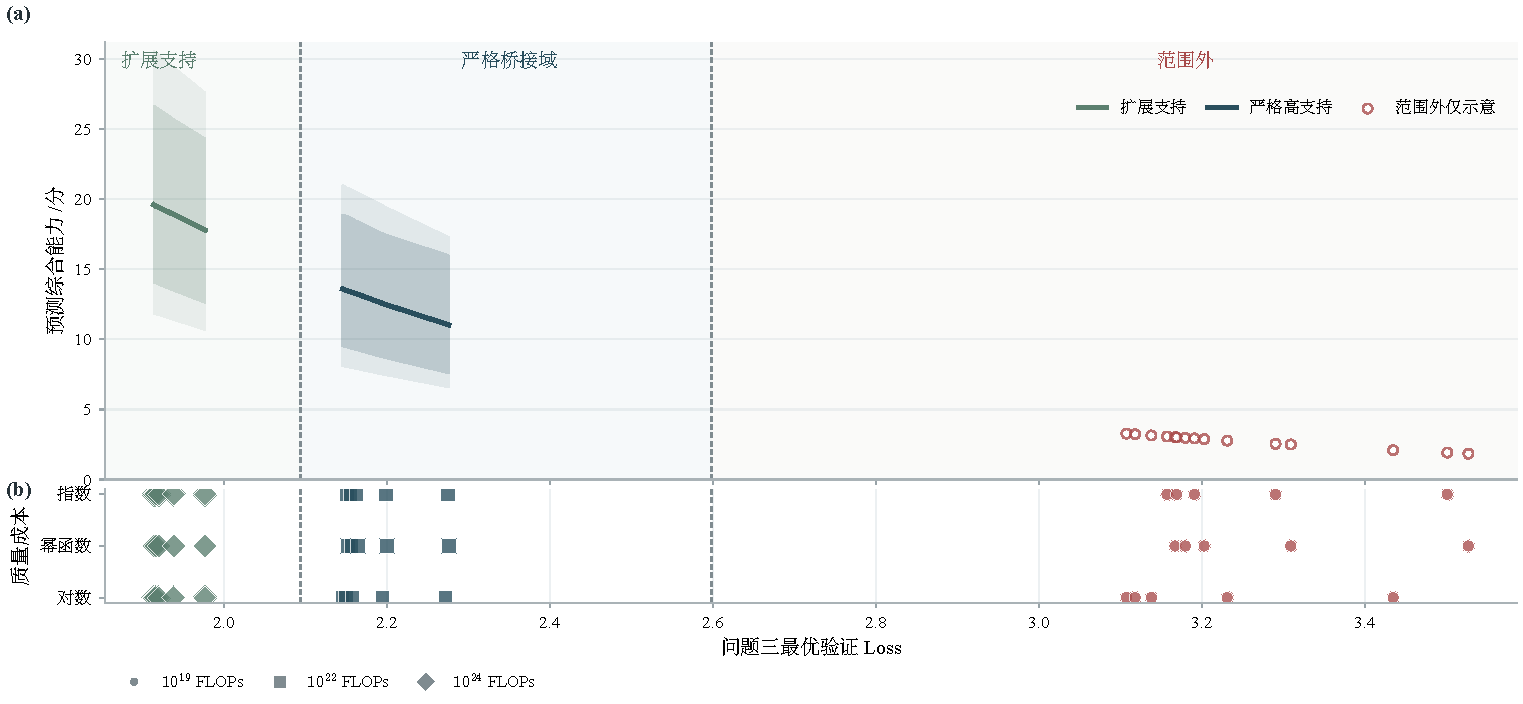
\includegraphics[width=0.98\textwidth]{images/no4/P4_F03_问题三Loss到综合能力映射.pdf}
  \caption{问题三最优 Loss 到综合能力的局部桥接映射}
  \label{fig:p4_p3_mapping}
\end{figure}

\begin{table}[htbp]
\centering
\caption{4096上下文下问题三最优Loss到综合能力的映射}
\label{tab:p4_p3_mapping}
\small
\setlength{\tabcolsep}{4.5pt}
\begin{tabular}{llrrrl}
\toprule
质量成本 & 预算/FLOPs & 最优 Loss & 能力中位数 & $80\%$ 区间 & 桥接支持 \\
\midrule
指数 & $10^{19}$ & $3.16898$ & $3.00$ & $[1.68,6.26]$ & 范围外，有限证据 \\
指数 & $10^{22}$ & $2.15491$ & $13.39$ & $[9.37,18.68]$ & 高支持 \\
指数 & $10^{24}$ & $1.91601$ & $19.51$ & $[14.02,26.56]$ & 扩展支持 \\
\midrule
幂函数 & $10^{19}$ & $3.17962$ & $2.97$ & $[1.63,6.24]$ & 范围外，有限证据 \\
幂函数 & $10^{22}$ & $2.15634$ & $13.36$ & $[9.35,18.63]$ & 高支持 \\
幂函数 & $10^{24}$ & $1.91611$ & $19.51$ & $[14.02,26.56]$ & 扩展支持 \\
\midrule
对数 & $10^{19}$ & $3.11805$ & $3.22$ & $[1.83,6.63]$ & 范围外，有限证据 \\
对数 & $10^{22}$ & $2.14975$ & $13.49$ & $[9.46,18.80]$ & 高支持 \\
对数 & $10^{24}$ & $1.91567$ & $19.52$ & $[14.03,26.57]$ & 扩展支持 \\
\bottomrule
\end{tabular}
\end{table}

表~\ref{tab:p4_p3_mapping} 表明，三种质量成本在中、高预算下映射出的综合能力非常接近，这是因为问题三的质量变量达到上界后，最优 Loss 主要由参数量和训练 Token 数决定。低预算方案的 Loss 高于 C6 完整支持上界，因此能力值仅用于回答题设情景，不能视为有直接观测支撑的精确预测。不确定性分解还显示，以指数成本、$10^{19}$ FLOPs 为例，上游 Loss 的 $80\%$ 映射宽度仅为 $0.078$ 分，而桥接不确定性宽度为 $4.687$ 分，说明结论的不确定性主要来自 Loss--Benchmark 映射而不是问题三优化器。

\subsection{模型求解}

\subsubsection{动力学能力前沿}

\subsubsection{条件分位模型}

能力前沿关注给定训练规模和时点下较优模型能够达到的水平，因此采用 $\tau=0.90$ 条件分位而非条件均值。分位回归能够直接刻画条件分布的高分位\cite{koenker1978quantiles}。令 $Y_i=g_{\epsilon}(S_i^{\mathrm{avg}})$，$x_i=\log_{10}C_i$，并将 $x_i$ 标准化为 $\widetilde x_i$，建立
\begin{equation}
Q_{\tau}(Y_i\mid x_i,t_i)
=\beta_0+\beta_C\widetilde x_i+a_{m(i)},
\qquad \beta_C\ge0,
\label{eq:p4_frontier}
\end{equation}
其中 $a_{m(i)}$ 为提交月份对应的非规模状态。主模型不同时放入 $C,N,D$，以避免 $C\approx6ND$ 引起机械共线；参数量模型 M-N 和参数--数据模型 M-ND 仅作机制诊断。

月度状态采用低自由度局部线性动力学
\begin{equation}
a_m=a_{m-1}+v_{m-1}+\eta_m,
\qquad
v_m=v_{m-1}+\zeta_m.
\label{eq:p4_state}
\end{equation}
数值实现用平滑 pinball 损失，并对状态的一阶与二阶差分施加惩罚。平滑强度 $\lambda$ 与未来状态斜率的局部权重 $\rho$ 只根据 $3$ 个月和 $6$ 个月滚动预测起点回测选择，保证每一折只使用预测时点以前的数据\cite{hyndman2021forecasting}。最终选得 $\lambda=10000$、$\rho=0$，即在当前短面板下采用高度平滑的状态并以全局斜率作保守外推；标准化算力系数 $\widehat\beta_C=0.6852>0$。

图~\ref{fig:p4_compute_frontier} 将确认性 pretrained 样本、平滑状态轨迹与算力方向置于同一坐标系中。该图的作用不是把相关性包装为因果性，而是直观核对：在控制观测期后，较高训练算力与较高动力学能力状态保持一致方向，且前沿外推没有脱离历史样本的局部支撑。

\begin{figure}[H]
  \centering
  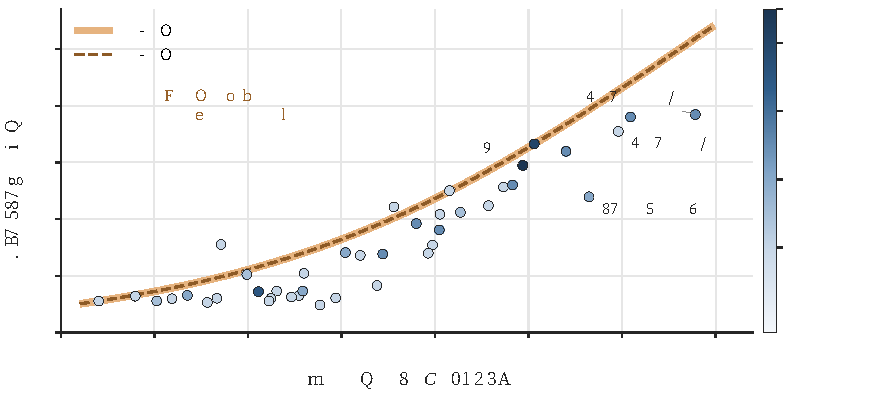
\includegraphics[width=0.94\textwidth]{images/no4/P4_F04_训练算力与动力学能力前沿.pdf}
  \caption{确认性 pretrained 样本的训练算力与动力学能力前沿}
  \label{fig:p4_compute_frontier}
\end{figure}


\subsubsection{求解与联合不确定性传播}

问题四从数据审计到前沿预测的完整计算过程归纳为算法~\ref{alg:p4_pipeline}。

\begin{algorithm}[H]
\caption{分层证据融合与动力学能力前沿预测}
\label{alg:p4_pipeline}
\begin{algorithmic}[1]
\Require C1--C6、C8，问题三冻结情景，分位集合 $\{0.85,0.90,0.95\}$，算力情景集合 $\{1,0.5,0.25\}$
\Ensure 综合能力、桥接结果、贡献分解与 $12/24$ 月前沿区间
\State 核验附件哈希、字段和子集关系，执行版本级去重与 C1/C2--C4 实体匹配
\State 按开放权重证据和模型类型构造确认性 pretrained 前沿面板
\State 由式~\eqref{eq:p4_average_score} 重建综合能力，并按式~\eqref{eq:p4_bbh} 复算 BBH
\ForAll{综合能力与六项任务目标}
    \State 对四类单调桥接执行来源族留一验证，并按一个标准误差规则选模
    \State 配对重采样问题三 Loss 与桥接来源族，输出支持域标签和能力区间
\EndFor
\State 滚动回测选择 $\lambda$ 与 $\rho$，拟合三条动力学分位前沿
\State 在模型家族簇与连续月份块上联合 bootstrap，并重估历史贡献
\State 按 C4 证据层构造月度算力前沿，在每次抽样中重估截止端点与增速
\ForAll{算力情景与预测时长}
    \State 预测三条分位前沿，对交叉分位执行单调重排并同步更新 link 与得分
\EndFor
\State 检查上游隔离、单调性、Shapley 闭合、分位次序、外推标签和复现性
\end{algorithmic}
\end{algorithm}

历史贡献的不确定性以模型家族为横截面簇、以连续月份为时间块进行重采样；未来预测还在每个抽样中重新估计算力端点、增长率和算力测量误差。时间相关数据采用块 bootstrap 的依据见文献\cite{kunsch1989bootstrap}。三条分位在每个抽样内部联合拟合，若发生交叉，则通过单调重排恢复 $q_{0.85}\le q_{0.90}\le q_{0.95}$\cite{chernozhukov2010quantile}，并由各自重排后的抽样计算区间。

\subsection{结果分析与模型验证}

\subsubsection{规模与非规模残余贡献}

选取确认性面板首末可用月份 $t_0=\text{2024-06}$、$t_1=\text{2025-01}$，并以各月训练算力的 $0.90$ 分位 $x_0,x_1$ 代表前沿规模。记 $F(x,t)$ 为式~\eqref{eq:p4_frontier} 经式~\eqref{eq:p4_link} 逆变换后的能力分。由于模型非线性，先替换规模和先替换时间会产生不同的边际增量，故采用两因素 Shapley 路径平均\cite{shapley1953value}：
\begin{align}
\Delta_{\mathrm{scale}}
&=\frac12\left\{F(x_1,t_0)-F(x_0,t_0)
+F(x_1,t_1)-F(x_0,t_1)\right\},\label{eq:p4_scale_contribution}\\
\Delta_{\mathrm{tech}}
&=\frac12\left\{F(x_0,t_1)-F(x_0,t_0)
+F(x_1,t_1)-F(x_1,t_0)\right\}.\label{eq:p4_tech_contribution}
\end{align}
两项必须满足
\begin{equation}
\Delta_{\mathrm{scale}}+\Delta_{\mathrm{tech}}
=F(x_1,t_1)-F(x_0,t_0).
\label{eq:p4_shapley_closure}
\end{equation}

分解结果见表~\ref{tab:p4_contribution}。中心估计的总变化为 $4.6182$ 分，其中规模扩张相关贡献为 $4.6183$ 分，非规模残余贡献为 $-0.0001$ 分。后者的 $80\%$ 区间跨越零，bootstrap 正号概率仅为 $0.528$，因此当前七个月现代面板不能识别稳定的非规模方向。本文不把接近零的中心残余解释为“技术没有进步”，而是认为在现有样本、口径和高度平滑的状态模型下，无法从规模项之外分离出稳定增量。

\begin{table}[htbp]
\centering
\caption{2024年6月至2025年1月的能力前沿贡献分解}
\label{tab:p4_contribution}
\small
\setlength{\tabcolsep}{8pt}
\begin{tabular}{lrrr}
\toprule
分解量 & 中心估计/分 & $80\%$ 区间/分 & $95\%$ 区间/分 \\
\midrule
能力总变化 & $4.6182$ & $[2.8418,5.6627]$ & $[2.5333,6.6860]$ \\
规模扩张相关贡献 & $4.6183$ & $[2.8407,5.6644]$ & $[2.5325,6.6868]$ \\
非规模残余贡献 & $-0.0001$ & $[-0.0018,0.0037]$ & $[-0.0027,0.0053]$ \\
\bottomrule
\end{tabular}
\end{table}


图~\ref{fig:p4_contribution_joint} 进一步给出两类贡献在联合不确定性下的分布。由于非规模项中心值略为负，普通百分比会出现符号反转或近零分母问题，故正文统一报告绝对贡献与绝对份额；规格与长期历史方向敏感性在本节末集中讨论。

\begin{figure}[H]
  \centering
  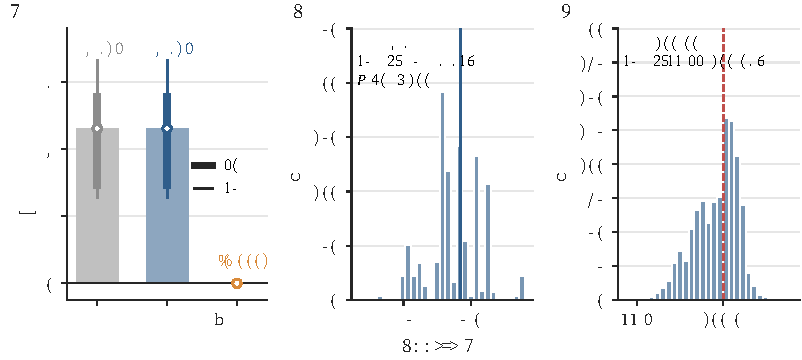
\includegraphics[width=0.80\textwidth]{images/no4/P4_F05_规模与非规模贡献联合分布.pdf}
  \caption{规模贡献与非规模残余贡献的联合分布}
  \label{fig:p4_contribution_joint}
\end{figure}

\subsubsection{算力放缓情景与未来能力前沿}

\subsubsection{算力端点与增长情景}

训练算力只使用预测截止日以前、开放权重、语言模型且证据方法为直接报告、运算计数或硬件估计的 C4 记录。算力估计的证据层、上下界和置信度处理遵循 Epoch AI 对训练算力估计方法的说明\cite{epoch2025computeestimation}；由 Benchmark 反推的算力不得再用于 Benchmark--算力关系，以避免循环论证。

同一家族同一月份先保留算力前沿版本，再在近 $24$ 个月的家族月面板上估计加权 $0.90$ 分位。稳健局部线性趋势给出截止月端点
\begin{equation}
x_{C,0}=25.092,\qquad
r_C=0.759\ \log_{10}(\mathrm{FLOPs})/\text{年},
\label{eq:p4_compute_growth}
\end{equation}
其中截止月原始月前沿为 $24.356$，最近三个月中位前沿为 $24.544$。端点使用截止月趋势拟合值而非全样本无时间条件分位，并在每个 bootstrap 抽样中与增速一同重估。

设算力增速保留系数 $\kappa\in\{1,0.5,0.25\}$，预测 $h$ 个月后的算力为
\begin{equation}
x_C(h;\kappa)=x_{C,0}+\kappa r_C\frac{h}{12}.
\label{eq:p4_compute_scenario}
\end{equation}
三种情景分别表示延续近期趋势、中度放缓和强度放缓。能力前沿由式~\eqref{eq:p4_frontier} 在未来月份的状态外推与式~\eqref{eq:p4_compute_scenario} 联合给出。

图~\ref{fig:p4_compute_scenarios} 将历史月度算力前沿与三条未来路径并列展示。本文缩放的是未来对数增长率，而不是把既有算力水平机械折减。

\begin{figure}[H]
  \centering
  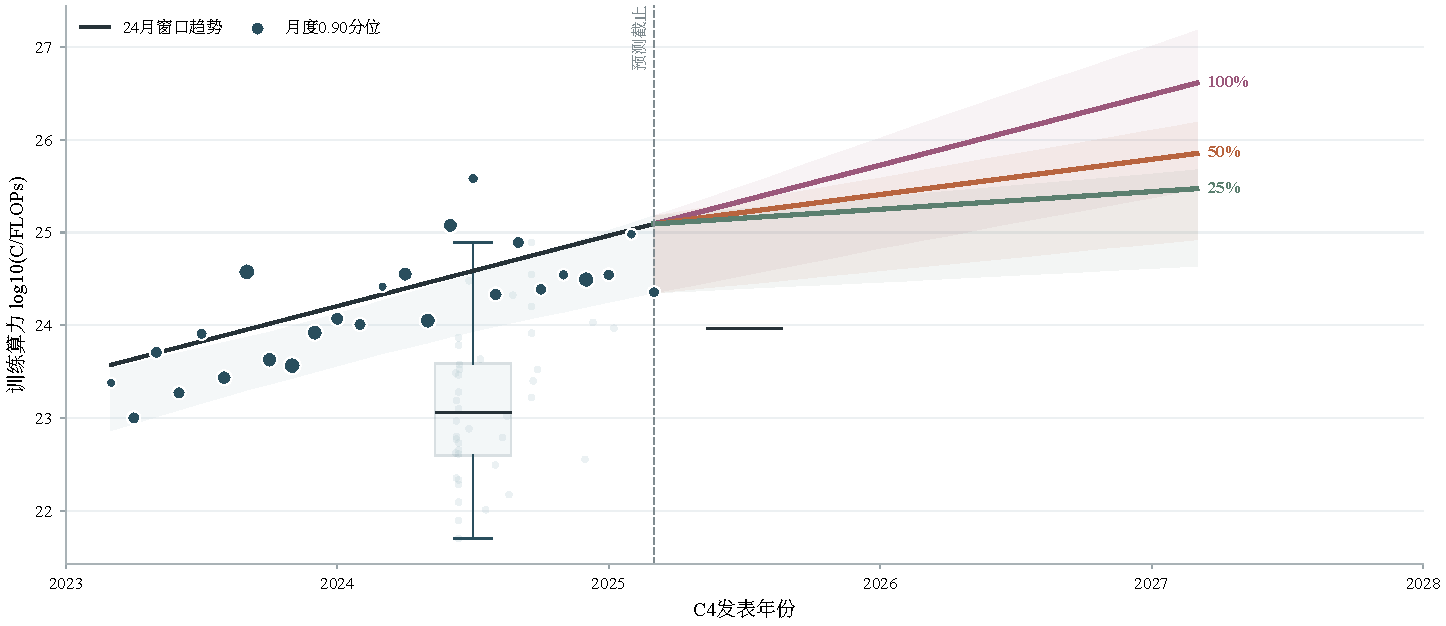
\includegraphics[width=0.98\textwidth]{images/no4/P4_F06_训练算力趋势与放缓情景.pdf}
  \caption{训练算力历史趋势与三种增长放缓情景}
  \label{fig:p4_compute_scenarios}
\end{figure}


\subsubsection{12个月与24个月预测}

主分位 $\tau=0.90$ 的结果见表~\ref{tab:p4_forecast}。全部区间同时包含历史前沿参数、未来状态斜率、算力端点、算力增速与算力测量误差；预注册 $1000$ 次联合抽样中获得 $999$ 次有效预测。

\begin{table}[htbp]
\centering
\caption{不同算力增速情景下的0.90能力前沿预测}
\label{tab:p4_forecast}
\small
\setlength{\tabcolsep}{6pt}
\begin{tabular}{lrrrr}
\toprule
算力情景 & 时长/月 & 前沿中心值 & $80\%$ 区间 & $95\%$ 区间 \\
\midrule
延续趋势（$\kappa=1$） & $12$ & $65.74$ & $[47.15,78.37]$ & $[40.25,86.09]$ \\
延续趋势（$\kappa=1$） & $24$ & $77.15$ & $[57.30,90.47]$ & $[47.49,95.29]$ \\
中度放缓（$\kappa=0.5$） & $12$ & $59.16$ & $[41.91,69.45]$ & $[36.47,77.85]$ \\
中度放缓（$\kappa=0.5$） & $24$ & $65.74$ & $[47.15,78.36]$ & $[40.25,86.08]$ \\
强度放缓（$\kappa=0.25$） & $12$ & $55.72$ & $[39.55,64.64]$ & $[34.60,72.52]$ \\
强度放缓（$\kappa=0.25$） & $24$ & $59.16$ & $[41.91,69.44]$ & $[36.47,77.85]$ \\
\bottomrule
\end{tabular}
\end{table}

图~\ref{fig:p4_future_frontier} 把表中六个点预测扩展为连续能力前沿。阴影区同时反映动力学状态、桥接模型和区组自助法的不确定性；放缓情景不仅压低中位前沿，也延后达到高能力区间的时间。

\begin{figure}[H]
  \centering
  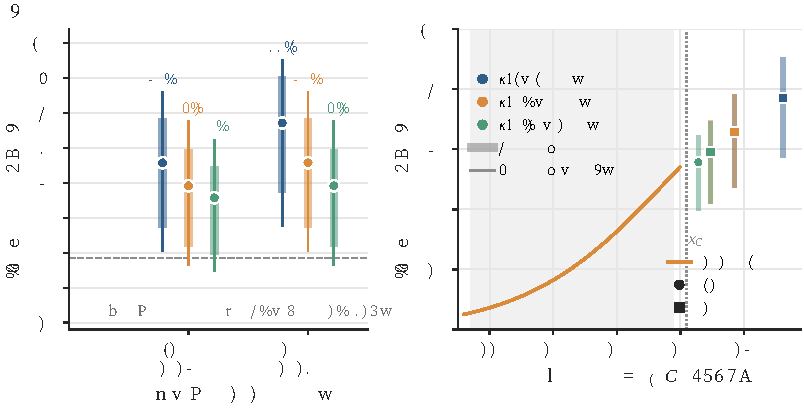
\includegraphics[width=0.96\textwidth]{images/no4/P4_F07_算力放缓下的未来能力前沿.pdf}
  \caption{算力增长放缓情景下的未来综合能力前沿}
  \label{fig:p4_future_frontier}
\end{figure}

预测结果具有清晰的情景递进性：算力增速越低、预测期越短，能力前沿越低；中度放缓 $24$ 个月与趋势延续 $12$ 个月的算力增量相同，因而前沿中心值均约为 $65.74$。然而，$12$ 个月结果已经超出同口径历史面板，必须标记为外推；$24$ 个月则属于长期外推。表中区间较宽，说明点预测不能脱离情景、区间和数据截止日单独使用。

\subsubsection{回测、数值验证与适用边界}

滚动起点回测在 $3$ 个月和 $6$ 个月步长上分别完成 $4$ 个有效起点。与 M-time 和 M-scale 基线比较，M-C 相对最佳基线 M-scale 的平均 pinball loss 差为 $0.00121$，配对标准误为 $0.00123$，未劣化超过一个标准误差，满足预注册放行条件。该回测只能检验短期排序和模型失效，不能被解释为对 $12/24$ 月外推的直接验证。

图~\ref{fig:p4_backtest_uncertainty} 同时呈现滚动回测误差和桥接区间宽度，避免仅用一条拟合曲线掩盖两类主要误差来源。近端回测支持方向稳定，但远端区间仍主要受外推距离和可迁移性假设支配。

\begin{figure}[H]
  \centering
  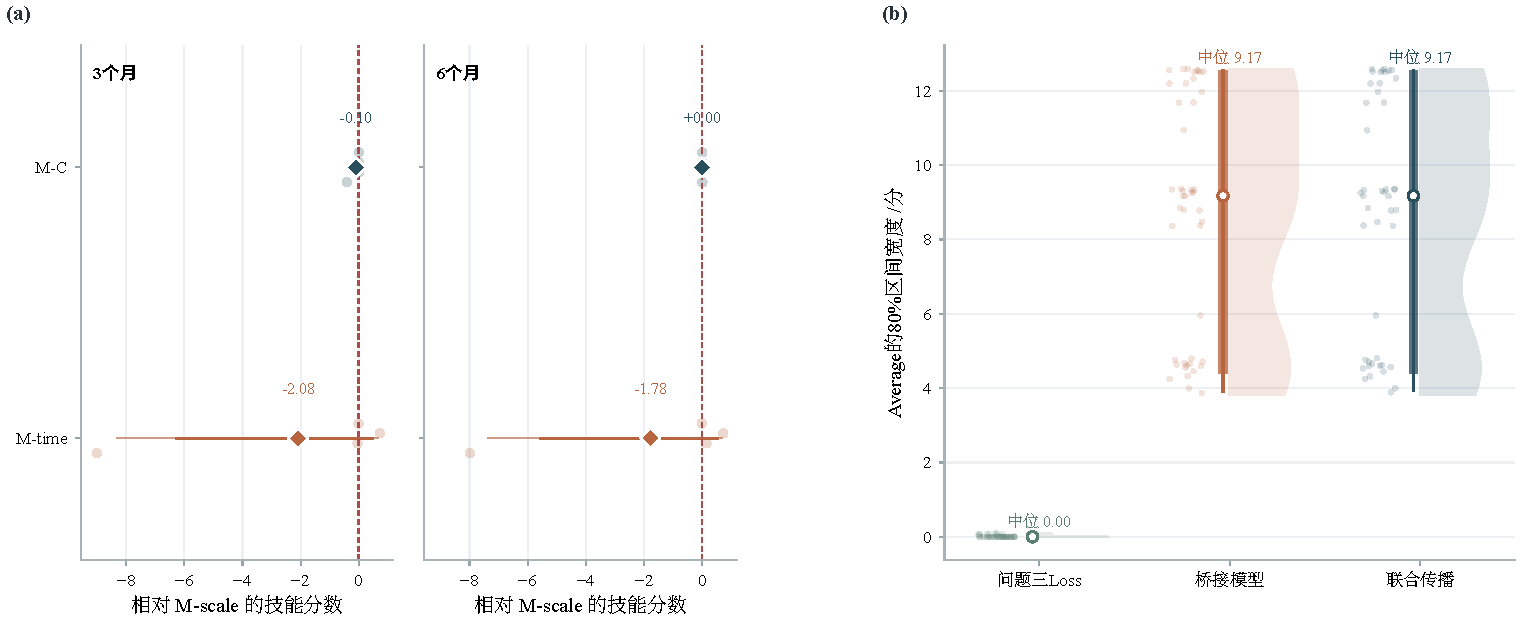
\includegraphics[width=0.96\textwidth]{images/no4/P4_F08_滚动回测与桥接不确定性.pdf}
  \caption{滚动回测误差与桥接不确定性诊断}
  \label{fig:p4_backtest_uncertainty}
\end{figure}


联合数值验收得到以下结果：全部桥接在稠密 Loss 网格上无单调违反；问题三 $45$ 个情景数量和标签保持不变，且进入历史训练集的数量为零；分数与 link 的最大不一致为零；三条分位在中心预测和抽样内均经重排保持有序；Shapley 在 link 与得分尺度的最大闭合误差为 $5.55\times10^{-17}$；相同配置连续运行两次的中心结果最大差为零。最终验收为 $29$ 项通过、$1$ 项警告、$0$ 项失败，数据、桥接、贡献分解、预测和总体五个接口均通过。唯一警告来自 MATH hard 逐任务重算未达到 $95\%$ 精确复现门槛，已通过只采用 BBH 正式证据完成降级处理。


\subsection{敏感性、适用边界与本问输出}

\subsubsection{贡献分解规格敏感性}

主口径采用严格 pretrained 样本、证据导向综合分数、发布时间轴、$\epsilon=1.5$ 和区组长度 3。分别改变样本边界、能力口径、时间轴、前沿容差与自助区组长度后，图~\ref{fig:p4_contribution_sensitivity} 中规模系数仍保持为正。不同设定会改变增量水平，但不改变“规模项主导、非规模残余缺乏稳定方向”的中心判断。

\begin{figure}[H]
  \centering
  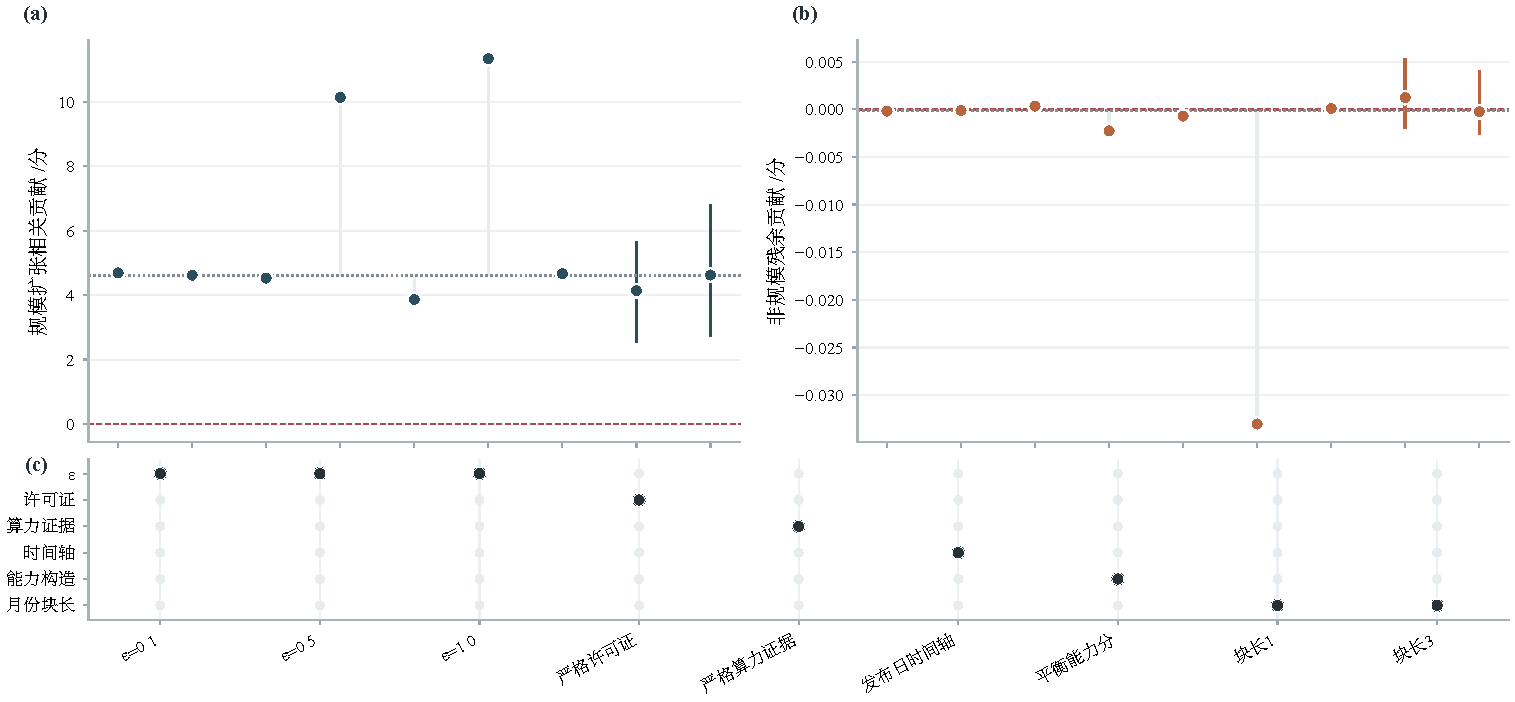
\includegraphics[width=0.98\textwidth]{images/no4/P4_A02_贡献分解规格敏感性.pdf}
  \caption{规模与非规模贡献分解的规格敏感性}
  \label{fig:p4_contribution_sensitivity}
\end{figure}

\subsubsection{长期历史方向敏感性}

2023--2024 年长期窗口仅包含 C3 与 C4 两个不同代际前沿点，因而只能承担方向核验。图~\ref{fig:p4_c3_sensitivity} 显示，引入 C3 历史信息没有推翻主样本的算力正向方向，但区间明显更宽、逐家族删除后符号不稳定，故不并入主估计。

\begin{figure}[H]
  \centering
  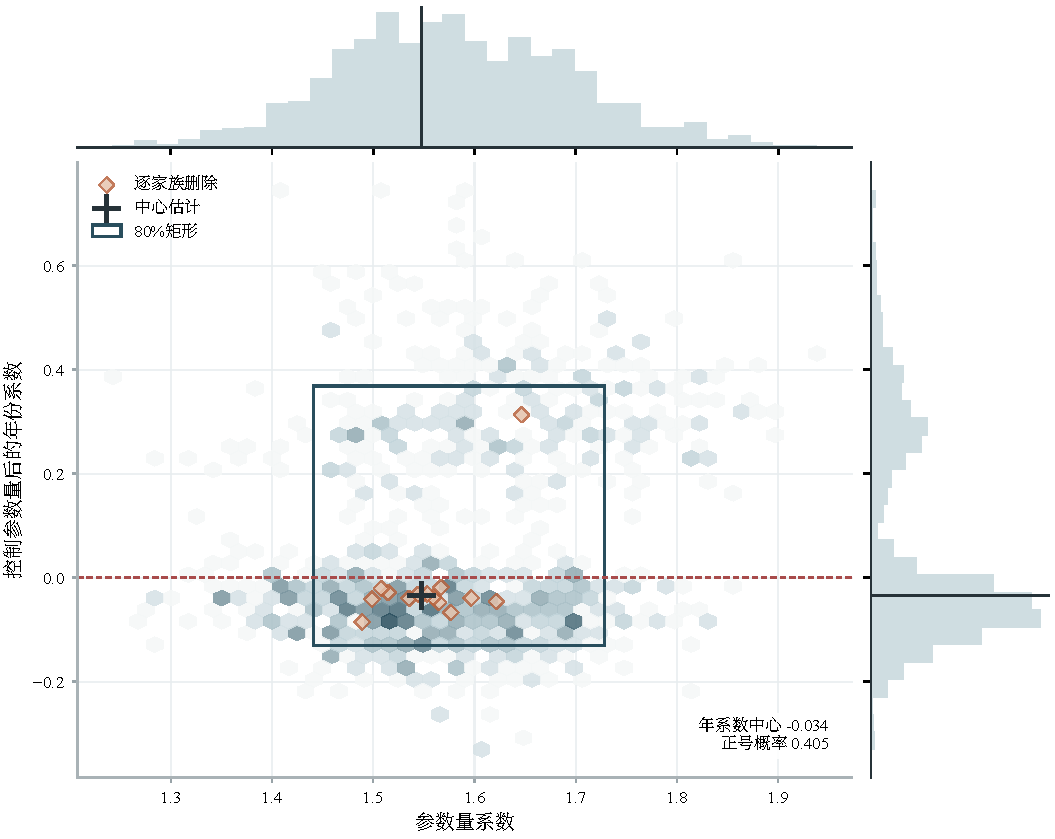
\includegraphics[width=0.80\textwidth]{images/no4/P4_A03_C3历史方向敏感性.pdf}
  \caption{引入 C3 历史信息后的方向敏感性}
  \label{fig:p4_c3_sensitivity}
\end{figure}

本问的适用边界有三点：第一，结论适用于公开可确认的 pretrained 前沿，不等同于对闭源训练过程的完全解释；第二，12/24 月结果是条件性情景预测，不是无条件点预测；第三，问题三样本只在训练后 Loss 的局部支撑域内用于桥接，域外情景仅用于风险提示。最终输出包括综合能力重建、算力--能力动力学前沿、规模与非规模贡献分解、三类算力放缓情景，以及相应的回测和敏感性证据。

综上，问题四在统一能力口径下完成了 Loss--Benchmark 映射、历史贡献分解与未来前沿预测。现有证据表明，2024 年 6 月至 2025 年 1 月的能力增量主要与训练规模扩张相关，控制规模后的非规模残余尚无稳定方向；若近期算力对数增速分别保留 $100\%$、$50\%$ 和 $25\%$，则 $24$ 个月后的 $0.90$ 能力前沿中心值约为 $77.15$、$65.74$ 和 $59.16$。这些结果是给定开放口径、数据截止日和算力情景下的条件预测，而不是确定性或因果性结论。
